\section{Gründungsfest WS 2023/24}
\sectionmark{Gründungsfest WS 2023/24}


\begin{figurehere}
		\begin{center}
			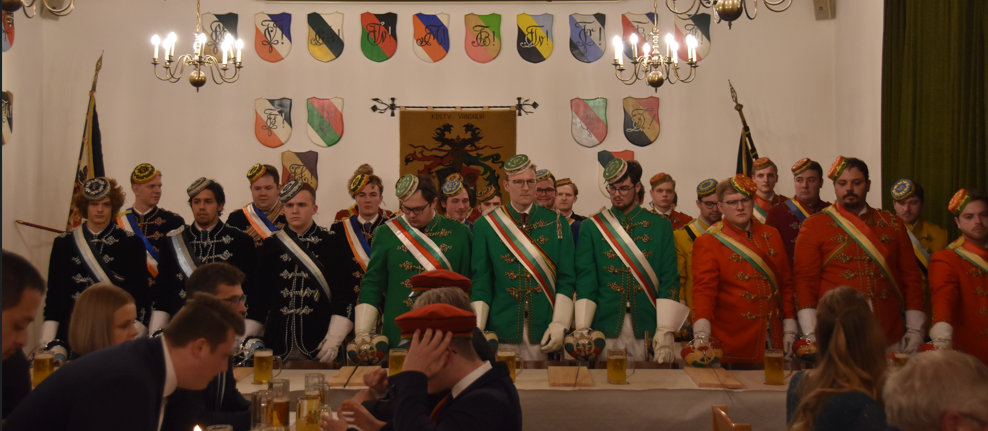
\includegraphics[width=0.8\linewidth]{./Bilder/1.2 Gründungsfest/1.corona.png} 
		\end{center}
	\end{figurehere}
	
\begin{multicols}{2}
Liebe Bundesbrüder,

vom 24. bis zum 26. November letzten Jahres fand unser 119. Gründungsfest statt. Aus aller Welt strömten zu dieser Festlichkeit Bundesbrüder herbei, und wir durften auch eine größere Zahl an Gästen und Cartellbrüdern willkommen heißen.

Den Auftakt machte am Freitag der traditionelle Begrüßungsabend, der unsere Erwartungen bei Weitem übertraf. Mit über siebzig Anmeldungen und etwa achtzig tatsächlich Anwesenden war der Saal gut gefüllt. Bereits bei den Vorbereitungen wurde klar, dass diese Teilnehmerzahl doch einige logistische Herausforderungen stellte, die jedoch leicht zu meistern waren. So war der Mitarbeiter an der Frischfischtheke eines Münchner Großhandels sichtlich erstaunt, als er bei einer unserer zwei Einkaufsfahrten die von uns gewünschte Menge Garnelen hörte. Am Donnerstagabend und den gesamten Freitag über standen immer mindestens ein halbes Dutzend Bundesbrüder in der Küche und bereiteten das Menü vor.

Für das Menü orientierte sich der Hohe Consenior, Derek Dominguez, an beliebten Gerichten aus seiner ecuadorianischen Heimat. Zur Vorspeise gab es eine Garnelenceviche, der man die hingebungsvolle Zubereitung durch die Bundesbrüder anmerkte. Insbesondere die dazu servierten Kochbananenchips waren bei den Bundesbrüdern sehr beliebt. Als Hauptgang wurden Fritadas serviert. Zu den in Öl gebackenen Schweinestückchen gab es eine bunte Auswahl an Beilagen wie gebratene Kochbananen und Kartoffeln. In Ecuador ist dies ein beliebtes Gericht auf Familienfeiern. Meist stehen die Speisen dabei auf großen Tellern oder Schüsseln auf dem Tisch, sodass sich jeder nach Belieben bedienen kann. Diese Darreichungsform dürfte, sofern sich das Gericht dafür eignet, auch für künftige Conseniores beim Einkauf von Töpfen und Geschirr eine Überlegung wert sein. Sie erleichtert das Auftragen und sorgt schnell für eine gelöste Stimmung an den Tischen. Nach einem von den Füxen verkauften Verdauungsschnaps fand das Essen mit der Nachspeise, dulce de higos, einen krönenden Abschluss. Zwar merkten wir beim Einkauf, dass gute Feigen nur noch bei den lokalen Gemüseläden in kleinen Mengen erhältlich waren und halb Schwabing danach durchsucht werden musste, doch letztlich gelang es dem Consenior, sehr schmackhafte, karamellisierte Feigen mit Sirup auf einer Scheibe Mozzarella zu zaubern. Im Anschluss ließen wir den Begrüßungsabend mit Tanz und dem einen oder anderen Getränk in der Füxenbar bei bester Stimmung ausklingen.

Am Samstag trafen sich die Aktiven bereits am frühen Vormittag, um mit einem Weißwurstfrühstück den Kater zu bekämpfen und sich für die nötigen Aufräum- und Umbauarbeiten zu stärken. Nicht jeder hatte es für nötig gehalten, die vergangene Nacht zumindest etwas zu schlafen, da es doch so einiges mit lange nicht gesehenen Bundesbrüdern auszutauschen gab. Der Schlafmangel machte sich bei manchem Redebeitrag auf den folgenden Conventen bemerkbar, die dennoch zügig vonstatten gingen. Nach einer kurzen Verschnaufpause traf man sich um 18:00 Uhr in St. Ursula zum gemeinsamen Besuch der Vorabendmesse. Mein Dank gilt hierbei unserem Bundesbruder AH David Theil, der die Messe in der ihm eigenen feierlichen Weise zelebrierte und uns unterstützt, obwohl er in seiner Stellung als Dekan häufig abends am Schreibtisch gebunden ist.

Pünktlich um 20 Uhr begann der Kommers als akademischer Höhepunkt des Gründungsfestwochenendes. Es dauerte wieder etwas länger als geplant, alle Chargierten aufzustellen, und es mussten noch einige Bänke organisiert werden, da ein paar Gäste keinen Sitzplatz hatten oder die für sie reservierten Plätze übersehen hatten. Neben vielen Cartellbrüdern und Bundesbrüdern samt ihren Familien sorgte auch die große Anzahl der Gastchargierten – trotz zweier kurzfristiger Absagen – für einen vollen Saal. So beehrten uns von außerhalb Abordnungen der e.V. K.D.St.V. Churtrier, e.V. K.D.St.V. Wiking Hamburg, deren ZMs wir in den letzten Semestern mehrfach bei uns begrüßen durften, sowie e.V. K.D.St.V. Franconia Czernowitz zu Erlangen. Aus München waren neben den Tuiskonen und Vindelikern auch der derzeitige MCV-Vorort, die K.D.St.V. Trifels, anwesend. Besonders erfreulich war die Anwesenheit zweier unserer Bandverbindungen, der K.D.St.V. Algovia Augsburg und der K.D.St.V. Oeno-Danubia Passau.

Nach der Begrüßung und einleitenden Worten meinerseits hielt der Festredner des Abends, der Erste Vizepräsident des Bayerischen Landtags a.D. Karl Freller, MdL, seine Rede. Im letzten Sommersemester sorgte die AfD mit einer Einladung einiger schlagender und rechter Verbindungen zu einer Kneipe im Landtag, bei der absichtliche Provokationen und schlechtes Verhalten inklusive gegenüber Journalisten stattfanden, für negative Schlagzeilen. Auch vor diesem Hintergrund war es mir eine besondere Freude, dass ein Mitglied des Landtagspräsidiums sich bereit erklärte, bei uns zu sprechen, obwohl unsere Anfrage mitten im Landtagswahlkampf kam. Karl Freller, der seit 1982 im Landtag sitzt und bis zur letzten Legislaturperiode der dienstälteste und jüngste Abgeordnete im Bayerischen Landtag war, hielt eine frei gehaltene Rede über den respektvollen Umgang miteinander und die Wichtigkeit, sich friedlich mit Andersdenkenden auseinanderzusetzen und füreinander einzustehen. Seine Rede war angesichts der Massaker vom 7. Oktober und des Missbrauchs der Parlamentsbühne durch die AfD in der letzten Legislaturperiode aufrüttelnd und bot uns einen interessanten Einblick. Man möge ihm verzeihen, dass er uns, als unerfahrener Korporationsgast, einmal als „Burschenschaftler“ ansprach; nach der Reaktion der Corona verstand er jedoch sofort den Unterschied. Ich bin erfreut, dass uns der Abend nicht nur eine interessante Rede bescherte, sondern auch dazu beitrug, katholische Verbindungen sichtbarer zu machen. Einen guten Eindruck über seine Person und sein Engagement, etwa im Holocaustgedenken, kann man auch auf Karl Frellers Webauftritt gewinnen.

Nach der Rede gab es als couleurstudentischen Höhepunkt des Abends drei Burschungen. Es war mir als Senior eine besondere Freude, den Bundesbrüdern Elia Strasser, Daniel Rampf und Raphael Frank das schwarz-rot-grüne Band umlegen zu dürfen. Die drei Neoburschen haben bereits in Chargen Erfahrungen gesammelt und werden unsere Verbindung in den kommenden Semestern sicherlich prägend mitgestalten.

Erfreulich war zudem, dass der Kommers trotz des voll besetzten Saals in guter, aber nicht ausufernder Stimmung verlief. Auch dank der Mithilfe der Bundesbrüder in der Corona konnte er zügig und in angemessenem Rahmen stattfinden. Dies tat der Stimmung keinen Abbruch, und so wurde bis in die frühen Morgenstunden die amicitia gelebt und das eine oder andere Bier bei guten Gesprächen getrunken.

Am Sonntag traf man sich mittags adh, um das Gründungsfest im gemütlichen Beisammensein ausklingen zu lassen. Gut zwei Dutzend Bundesbrüder spazierten bei goldenem Herbstwetter zum „Georgenhof“, wo man – bei inzwischen recht hohen Preisen – eine wunderbare bayrische Stärkung zu sich nahm. Während sich viele der von außerhalb angereisten Bundesbrüder nun verabschieden mussten, ging der Rest am letzten Sonntag des Kirchenjahres zum frisch eröffneten Christkindlmarkt auf dem Stachus. Leider erwies sich dieser als recht überlaufen, und die 10 \euro ~für eine kleine Tasse Glühwein sowie die einbrechende Kälte luden nicht zum Verweilen ein. Auch das wiederholte Aussenden von Echolokationssignalen konnte einen nicht anwesenden Bundesbruder nicht aufspüren. So beschloss man, bis in die frühen Abendstunden eine kleine Tour durch die Münchner Kneipen zu machen. Abschließend lässt sich sagen, dass es künftig eine Überlegung wert wäre, bei einem der jährlichen Feste am Sonntagmorgen den Gottesdienst zu besuchen, um die Anwesenheit der AHAH und ihrer Familien beim Ausklang sicherzustellen und gleichzeitig einen entspannteren Samstagnachmittag zu ermöglichen.

Mit bundesbrüderlichen Grüßen,

	%
	\begin{flushright}
		\hfill\emph{Konrad Schönleber RBo! Va!\\
Mathias Brezina Va!}
	\end{flushright}
	%	
\end{multicols}


%
%\begin{figurehere}
%	\begin{center}
%		\includegraphics[width=.8\linewidth]{Bilder/pios2}
%		\caption{Realer Aufbau} 
%	\end{center}
%\end{figurehere}